\section{System Architecture}

Our first step, after reading the description of our project, was to decide what kind of application or system would be best suited to tackle our requirements. The first thing that we gleaned from the specification was that some form of persistent storage would be required. For example, the user submitted scripts must be stored so that they can later be raced against new scripts and data used to rank the scripts must be recorded so that a leaderboard can be shown. It was also mentioned in our project's specification that we should use the Unity game engine for the physics simulation and visualisation of our vehicle races. These two requirements gave us a solid starting point for designing our system. Our first thought was to develop a stand alone Unity application to run on any desktop machine. This option would have required one machine to act as a server and manage the centralised data while the other machines communicate with it using networking code inside of Unity. It would also have meant we'd need to build a full user interface for uploading, editing and managing scripts inside of Unity. The more we thought about this the more we realised that these tasks would be a massive undertaking and highly difficult to achive in the time frame, due to our group's limited knowledge of Unity.

Once we began thinking about alternatives an obvious solution sprang to mind. A huge benifit of Unity is that it is highly portable and can be run on many different platforms. One of these platforms is the Unity Web Player, a browser plug-in that allows Unity applications to be run inside all modern web browsers. If we used the web player we would could pull all of the things that are difficult to do in Unity outside of the Unity application and into the web browser. Thus turning the task of creating an easy to use interface for uploading scripts into a web design problem, a domain that is a lot better suited to solve user interface tasks such as this. The Unity application is then only needed for running and visualising the races. Unity also provides features for communication with the web browser, in both directions, when running in the web player, making passing data to the Unity application at runtime easy. This design also reduces the complexity of the networking problems as now one machine can run a web-server and database, using standard web technologies, while client machines simply run a web browser, containing the Unity Web Player, and communicate with the server using standard web protocols.

\subsection{Component Diagram}

\tikzset{%
  block/.style    = {draw, thick, rectangle, minimum height = 3em, rounded corners,
    minimum width = 3.5em, align=center},
  sum/.style      = {draw, circle, node distance = 2cm}, % Adder
  %input/.style    = {coordinate},
  db/.style  = {draw, cylinder, shape border rotate=90, aspect=0.25},
  interface/.style    = {draw, thick, rectangle,
    minimum width = 4em, align=center},
}

\begin{center}
\begin{tikzpicture}[auto, thick, node distance=2cm, >=triangle 45]
	% Blocks of FRONT END:
	\draw
		node at (1, -1.7) [block] (unity) {Game \\ Objects}
		node [block, right of=unity, right=-0.25cm] (webplayer) {Unity \\ Webplayer}
		node [block, right of=webplayer, right=-0cm] (unityscript) {Unity \\ Script}
		node [block, right of=unityscript, right=-0.35cm] (ai) {AI\\Script}
		node [block, right of=ai, right=-0.5cm] (browser) {Browser}
		%node [sum, right of=input1] (suma1) {Unity}
	;
    	% Joining FRONT END:
	\draw[->] (browser) -- node {} (ai);
	\draw[->] (ai) -- node {} (unityscript);
	\draw[->] (unityscript) -- node {} (webplayer);
	\draw[->] (webplayer) -- node {} (unity);
	\draw[-] (webplayer) |- node[right=3.5cm, above] {\small Request Commands } ($(browser.north) + (0, 0.5)$);
	\draw[->] ($(browser.north) + (0, 0.5)$) -- node {} (browser);

	% Blocks of MIDDLE
	\draw
		node at (5.5,-4) [block, name=rest] {REST API}
	;

        % Blocks of BACK END
	\draw
	        node [block, below of=unity, below=2.3cm, name=express] {Express\\Router}
	        node [block, right of=express, right=0cm, name=passport] {Passport \\ Auth.}
	        node [db, below of=passport, below=0cm, name=mongo] {MongoDB}
	        node [interface, above of=mongo, above=-1cm, name=monk] {Monk Adapter}
	        node [block, right of=passport, right=0cm, name=routes] {Routes}
	        node [block, right of=routes, right=0cm, name=views] {Views}
	;
	% Joining BACK END
	\draw[->] (express) -- node {} (passport);
	\draw[->] (rest) -| node {} (express);
	\draw[->] ($(browser.south) + (-0.2, 0)$) |- node[left=2.25cm, below] {\small Request Page} (rest);
	\draw[-, dotted] (passport) -- node[below right] {} (monk);
	\draw[-] (monk) -- node {} (mongo);
	\draw[->] (passport) -- node {} (routes);
	\draw[->] (routes) -- node {} (views);
	\draw[-, dotted] (routes) |- node {} (monk);
	\draw[->] (views) -| node {} ($(browser.south) + (0.2, 0)$);

	% Boxing
	%\draw [color=gray,thick, dotted] ($(passport.north west)+(-0.2,0.2)$) rectangle ($(monk.south east)+(0.2,-0.2)$);
	\draw [color=gray,thick](-0.5,-3) rectangle (12.55,0);
	\node at (-0.5,0) [above=5mm, right=0mm] {\textsc{Front-End}};
	\draw [color=gray,thick](-0.5,-10.5) rectangle (12.55,-5);
	\node at (-0.5,-10.5) [below=5mm, right=0mm] {\textsc{Back-End}};
\end{tikzpicture}
\end{center}

\section{Back-end}
The architecture of our server revolves around providing a website to upload, manage and score AI scripts. We provide these services via a simple REST API, implemented with Node.js\cite{whynode} and its supporting libraries:
	\begin{itemize}
	        \item \textbf{Express}\cite{express} is a light-weight web application framework that supports the MVC design pattern using routes (controllers) and views.  
		\item \textbf{Passport}\cite{passport} handles authentication for our website. We currently use the 'local' package which provides account registration and login via our Mongo database. However, in the future we could easily slot in Facebook or Google packages to provide alternative login methods.	
		\item \textbf{Monk}\cite{monk} provides a simple adapter to access our Mongo database in JavaScript. It uses an asynchronous tactic of searching by a filter object (e.g. to find a user called Steve, you'd filter with a new user object with name Steve) combined with a closure to be invoked on the found objects. 
\begin{figure}[H]
\centering
\begin{lstlisting}[language=JavaScript]
router.get('/script/:name', function(req, res) {
    db.get('scriptcollection').findOne({scriptName:req.params.name},  
        function(e, doc) { res.send(doc.script, 200); }
    );
}
\end{lstlisting}
\caption{Example use of Express (router.) \& Monk (db.) to GET a script.}
\label{fig:getscript}
\end{figure}
		
		\item \textbf{Forever} solves one of the main limitations of Node.js: that in the event of an exception the website will crash and shut down. Forever is a simple way to keep a script, and thus the website it controls, operating continuously. In the event of an uncaught exception, server restart or otherwise fatal condition Forever will restart the website immediately. Forever also maintains a log of such circumstances to help track down the cause.
	\end{itemize}

\subsection{REST API}
Why use REST API?

Below you can see some example interactions with our REST API:\\

\begin{center}
\begin{tabular}{| l | l | l | l |}\hline
Route & Request &  Response & Explanation\\\hline\hline
/script & GET & View & Show the create new script page\\\hline
/script & POST & None & Store a new script to the server\\\hline
/script/DrEvil & GET & String & Get the code for script DrEvil [see Figure \ref{fig:getscript}]\\\hline
/edit/DrEvil & GET & View & Show the live edit script page\\\hline
/tournament & GET & View & Show the next tournament match\\\hline
/tournament & POST & View & Store the match result and show the next \\\hline
\end{tabular}
\end{center}

Comment on the table.

\subsection{MongoDB}
For our database persistence we use an open source, document based solution - MongoDB\cite{mongo}. Mongo provides fast, scalable data storage with rich, object based queriers.

Our main motivation for using MongoDB was the flexibility its schema-less design offered\cite{whymongo}. Rapidly prototyping new ideas and concepts is much more productive when the updating and deployment of database schemas can be ignored. During such development data entries can frequently gain and lose attributes, which requires no interaction with the database when Mongo is used. Furthermore, by using the Monk adapter we can implement our full back-end in a single language, JavaScript, without complicated SQL statements.

\begin{figure}[H]
\centering
\begin{tikzpicture}[node distance=7 em]
\node [entity] (person) {User};
\node [relationship] (has) [right of=person] {Owns};
\node [entity] (script) [right of=has] {Script};
\node [attribute] (email) [above of=person] {\key{Email}} edge (person);
\node [attribute] (pid) [below of=person] {Year?} edge (person);
\node [attribute] (pid) [below left of=person, above=0cm] {Degree?} edge (person);
\node [attribute] (pid) [left of=person, left=-0.6cm] {University?} edge (person);
\node [attribute] (pid) [above left of=person, above=-0.5cm] {Hash} edge (person);
\node [attribute] (pid) [above of=script] {\key{Name}} edge (script);
\node [attribute] (pid) [below of=script] {Code} edge (script);
\node [attribute] (pid) [above right of=script] {Language} edge (script);
\node [attribute] (pid) [below right of=script] {Rating} edge (script);
%Edge
\path[every node/.style={font=\sffamily\small}] (person) edge node [above] {0..N} (has);
\path[every node/.style={font=\sffamily\small}] (script) edge node [above] {1..1} (has);
\end{tikzpicture}
\caption{ER diagram for our data persistence.}
\label{fig:ER}
\end{figure}

From Figure \ref{fig:ER} you can see another justification for our use of NoSQL technologies: the relationship is very simple. Document based technologies such as Mongo can struggle to provide simple modelling of complicated relationships, in these situations SQL based implementations typically offer a better solution. 

\section{Browser Front-End}

For the browser front-end, i.e. website, we used three technologies : Jade, Bootstrap and the Ace editor.


\subsection{Jade}
As explained above, we chose to use the Node.js platform, and we next had to chose a template engine for it's web template system. We chose to use Node's default engine, Jade\cite{jade}, which is written in JavaScript and specifically a templating language for HTML. It simplifies writing web pages as it is less verbose than HTML, and allows template inheritance (demonstrated below) alongside other dynamic constructs such as conditionals and loops.
\vspace{-2mm}
\begin{figure}[H]
\centering
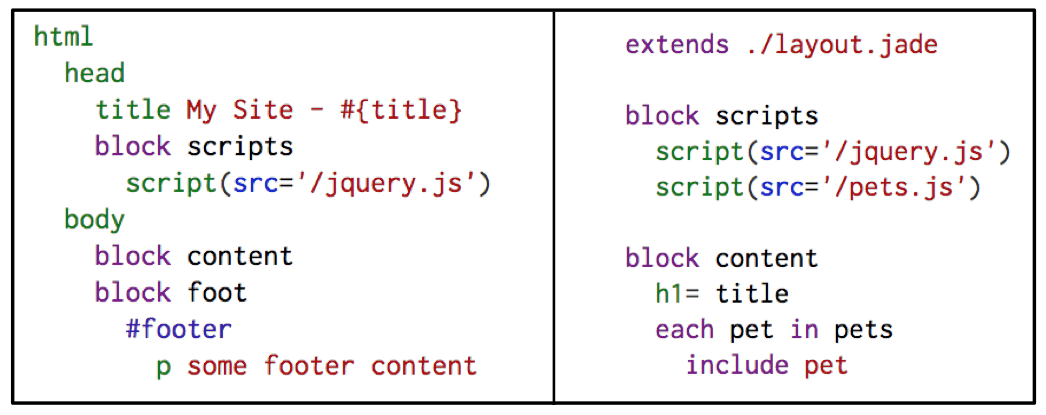
\includegraphics[scale=0.25]{jadeexample.png}
\caption{Jade template inheritance is simple and powerful.}
\end{figure}

\noindent Compared to other engines such as Swig and Hamljs, which have similar feature sets, Jade has had reported sluggish benchmarking performance \cite{benchmarks} (obviously some benchmarks can't be treated as gospel). However, performance was not a concern for us; templating engines are very rarely a system bottleneck, and the decision to use Jade was founded upon it's usability and readability.

\subsection{Bootstrap}
Given our limited experience using Jade/HTML and CSS, alongside our negligible artistic talent, we opted to use Twitter's Bootstrap to design our website. Bootstrap makes web design a breeze by providing the HTML and CSS templates for well-designed web components, including forms, buttons, navigation bars, JavaScript extensions and more. In particular, we used the Sandstone\cite{sandstone} template from Bootswatch (released under MIT license), demonstrated in the figure below. Although this may not give users with a particularly unique experience, it means providing users with a familiar experience that would allow them to utilise preconceived assumptions on how the website can be navigated - avoiding the need to explain the website explicitly.

\begin{figure}[H]
\centering

\includegraphics[width=0.5\textwidth]{sandstonetheme.png}
\caption{Bootswatch Sandstone theme sample.}
\end{figure}

\subsection{Ace}
Apart from the most cavalier advocates of text editors, programmers shudder at the idea of coding in a plain text area. To simplify the process of reading, writing and submitting scripts, we chose to use a web-based code editor. There are few open-source editors that can rival the performance, features and simplicity of Ace (a standalone editor written in JavaScript). Ace\cite{ace} is actively developed for use in the online Cloud9 IDE, yet can be embedded in any web page (see picture below) given its BSD license.

\begin{figure}[H]
\centering
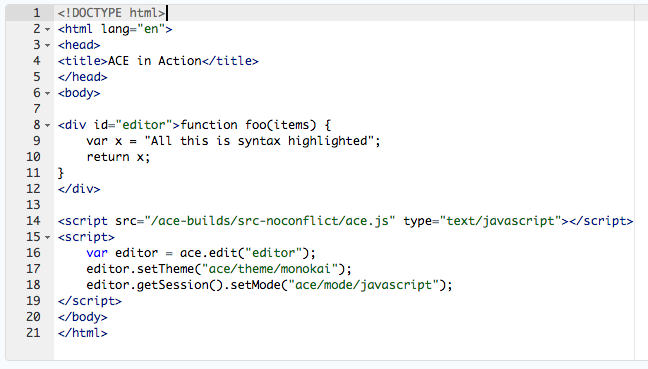
\includegraphics[width=0.75\textwidth]{aceeditorexample.png}
\caption{Ace editor containing code needed to embed in a web page.}
\end{figure}

\noindent By using Ace, users have JavaScript syntax highlighting, syntax error checking, searching/replace, automatic indentation etc. Not only does this improve the productivity of a user, which is important given the time pressures which may be faced if a queue forms at the G-Research careers fair stand; but it provides immediate feedback for those unfamiliar with JavaScript syntax, which may be the majority of users, reducing the likelihood of submitting broken scripts.

\subsection{Risks}

\subsubsection{Browser Cross-Compatibility}

It is rare for websites and web applications to function identically or appear the same across multiple web browsers, due to the varying compatibilities of even the most popular browsers - this can be problematic for many modern websites. We mostly spent time testing AI Racing Market on Google Chrome, yet tested on Mozilla Firefox and Safari occasionally. Needless to say, this does not replace proper cross-browser compatibility testing using the many tools (such as emulation environments) available to developers these days. However we did not deem this a significant risk, as G-Research employees should be able to iron out compatibility issues prior to a careers fair, installing and choosing the most functional browser in advance. With most of the well known browsers, it is likely that the user interface will simply appear jumbled yet remain functional.

\subsubsection{Mobile Compatibility}

At careers fair, may be nothing stopping user from submitting a script by their phone/tablet following using the handout etc.... (G-Research may encourage etc)... Compatibility!

\subsection{Challenges}
Solutions

\subsubsection{Streamlining User Interactions}

We didn't want users to dilly dally, see UI section

\subsubsection{Unity Web-player Loading Times}

On edit screen, as we will describe further in X, we load unity web player. THis is slow as fuck, and during development would freeze/some other excuse. Now we do X which somehow works...

\section{Unity Application {\color{blue} CHRISTOPHE}}
No external tech used except for a few of Unity's basic script assets, e.g. smooth follow cam.

Main design points:
Designing the Script API
Managing and recording race data e.g. checkpoints, hud
Comunication with browser i.e. starting race, where scripts are exectued, how many calls per frame

Unity applications are based around a system of scenes that can be switched between at runtime. We used this in our application to have a seperate scene for each racetrack we had built. As, in our case, each time the application is loaded only

\subsection{API Design}
The key component of the Unity application is the scripting API and our first step in its design was to decide how to give information about the race track so the user can complete a lap. We eventually settled on making this very simple for the user - we drew a line along the centre of the track and let the user set the speed of the car. Our API will automatically steer the car along the centre line at the set speed. Our reasoning on making steering so simple was that guiding the car around the track is the first and least interesting step and we did not want every user to spend the first few minutes writing the same line following script. However this caused races to disintegrate into a train of cars following the same line around the track where the car in first place at the start of the race will be the winner. We solved this creating two more lines for the cars to follow on either side of the centre line and providing API calls to switch to the line on the left or on the right. These calls can be used to overtake cars or to switch to the inside line of a corner.

Finally, we added a few more features which scripts can use to distinguish themselves: the distance to the next corner, the curvature of that corner and a ``boost'' ability which gives the car a large speed increase but may only be used every few seconds. A good script can make use of these features by boosting along straight sections and slowing down according to the sharpness of the corner.

\subsection{Race Data}

\subsection{Browser Communication}

\subsection{Risks}
Spending ages on

splines from timeboxed spikes section?

Anticipation \& Mitigation

\subsection{Challenges}
Designing the script API

Initially we had a very simplistic system of controlling and receiving environment information from the car.

steering and throttle control for control. Proximity sensors (ray casting) for position information.

Solutions

\subsubsection{Steering the Car}
To guide the car around the track we initially placed invisible walls along the edge of the track and created proximity sensors on either side of the car to measure the distance to these walls. The output of the sensors was used to steer the car toward the current lane. The main problem with this approach was that the cars would always drive forward even when pointing the wrong way after skidding or a crash causing the cars to drive the wrong way around the track.

We solved this problem by replacing the walls and proximity sensors with a spline along the centre of the track and keeping a target position on this spline. The car will always steer toward this target position and the target will always be a small distance in front of the car. This ensures that the car will always drive the right way along the track. Another advantage of the splines is that if two cars take a corner too quickly, the car moving moving faster will end up further from the track and therefore lose more time than the slower car. With the old approach, both cars would simply bounce off the walls and the faster car would not be penalised more than the slower car.

\subsubsection{Tournament Closing Conditions \& Ranking}
% Define "ranking of the cars" for the reader?
Users are able to submit scripts which cannot finish a race in a reasonable time or which will never finish e.g. cars which flip over in corners, cars which only drive backwards or stay at the start line and cars which override the default steering and go off track. So our tournament must be able to terminate a race before all cars have finished if necessary and still provide a good ranking of the cars.

We accomplished this by placing invisible checkpoints to split each track into short straight sections. We keep maintain the next checkpoint and the time since the last checkpoint was completed for each car. From this we can tell if a car has finished (when the last checkpoint in the race is completed for the third time) or if the car has timed out (if the last checkpoint was completed more than 30 seconds ago). The 30 second time limit is very generous and even a cautious script can easily complete each checkpoint in this time, so a car which times out will belong to an incorrect script. The tournament is ended when all cars have either completed the race or have timed out. Cars which completed the race will be ranked by their time while cars which have timed out will be ranked according to the number of checkpoints completed, if this is equal, then the straight line distance to the next checkpoint is used instead.

\section{User Interface Design}

\subsection{Design Philosophy}

At a a busy careers fair we expect students will have roughly 5-10 minutes sessions with AI Racing Market. Ideally students will have the chance to return and improve their scripts, yet this may be infeasible if there are a lot of interested students. Given students will be short on time, under pressure and likely new to the game, we focused on :
\vspace{-1mm}
\begin{enumerate} \itemsep -2pt 
\item Simplicity
\item Minimal Interactions
\end{enumerate}

We previously justified our use of Bootstrap by the provision of a familiar user experience. By providing the user with a simplistic and familiar interface, users need little explanation of website navigation and can simply focus on script editing and submission. 

An example of how we achieved this was a common navigation bar seen on each web page. This functions as a website backbone, providing the user with access to all of the website's  features. Our template engine, Jade, made this incredibly simple (as shown below); we wrote a basic navigation template that extended our generic Bootstrap layout, which could then be included within the other templates (in Node.js, these are called {\it views}). 

\begin{figure}[H]
\centering
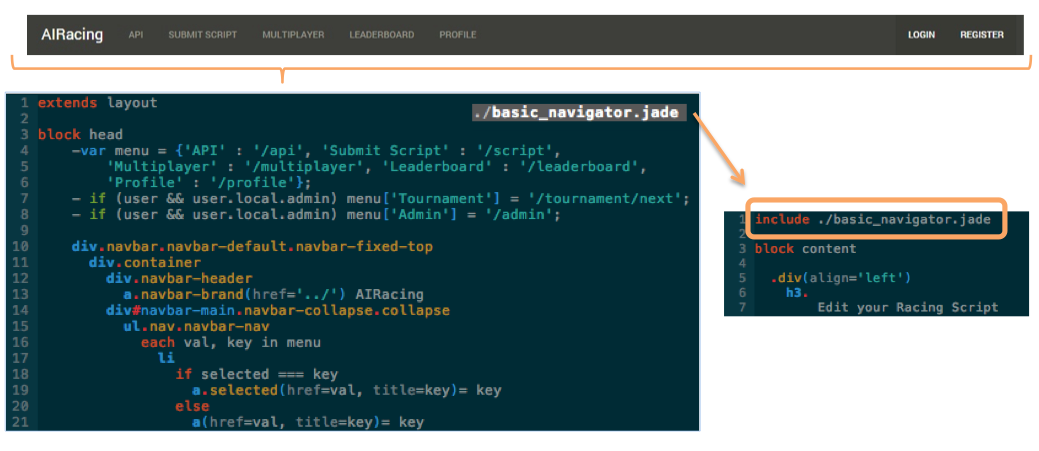
\includegraphics[width=\textwidth]{jadenavigator.png}
\caption{Jade navigator template included within each view.}
\end{figure}

\subsection{Anonymous Script Submission}

Few things kill the excitement of a new game like a lengthy registration process, especially when handing over your email could spell nothing but more email spam. Although we trust that G-Research wont spam students using AI Racing Market, or sell their email addresses to third parties, we designed the script submission such that the users did not have to register. Not only does reduce the interactions needed for a new user to get involved with racing, but it allows the users to remain anonymous, removing the concern that a poor performing script tied to their email address will result in G-Research immediately dismissing their application. As shown below, the user simply associates their work with a script name, and can immediately create a script.

\begin{figure}[H]
\centering
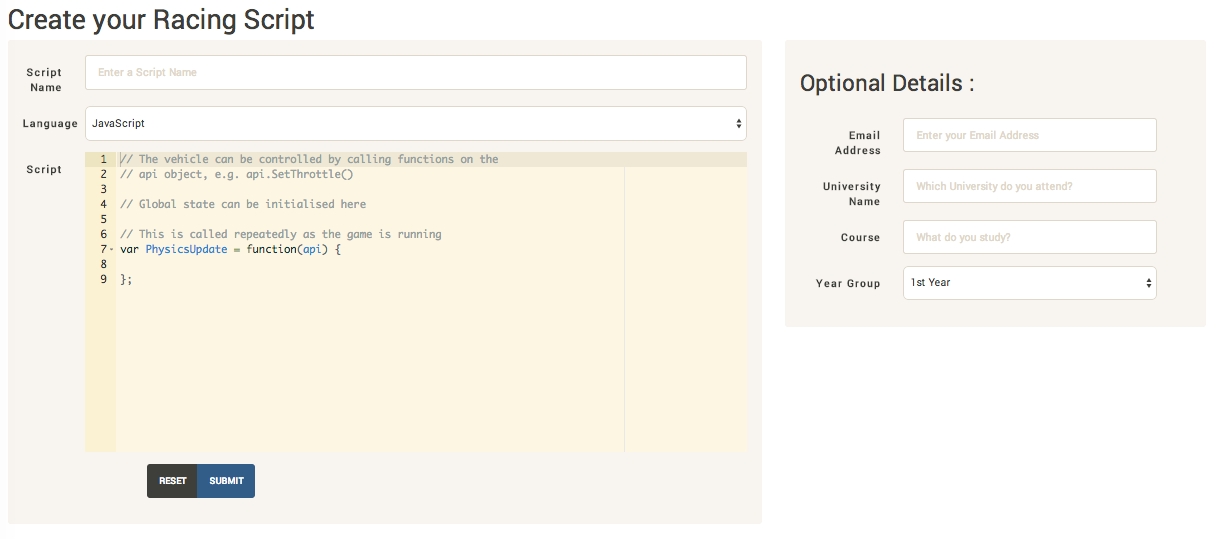
\includegraphics[width=0.8\textwidth]{anonymoussubmit.png}
\caption{Admins will see additional features on their navigation bar after logging in.}
\end{figure}

As we discuss later in this section, G-Research wants to harvest user data.  Therefore we added an ``Optional Details" panel on the right hand side of the script submission screen, allowing users to provide G-Research with information if they wish. If these details are submitted, they are not tied to an account or script until a user registers with the same email address. This means G-Research can recognize that a student has attended their careers fair stand, however their performance can't be scrutinised. If a user is already logged in and wants to submit a new script, they will face the same screen as shown above, excluding the optional details pane.

\subsection{Responsive Script Editing}

Clearly the script submission screen presented above is limited; it provides basic syntax checking, however users will have no feedback on how their scripts perform prior to racing in the tournament. If a user has registered, they can navigate to a more responsive editing mode by clicking on of their submitted scripts, listed on their profile (shown below).

\begin{figure}[H]
\centering
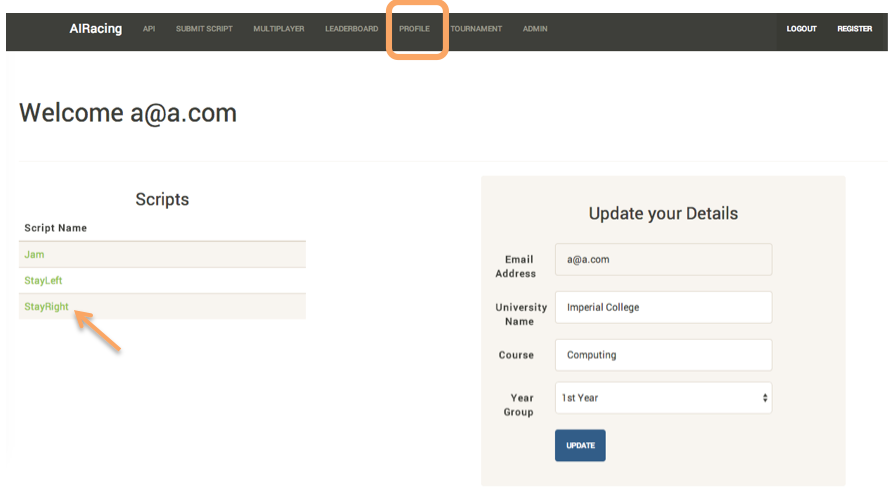
\includegraphics[scale=0.35]{profiletoedit.png}
\caption{Registered users have their scripts listed on their profile, these can be edited on click.}
\end{figure}

After selecting a script to edit, they are presented with not only an Ace editor, but a test race (shown below). Although the user cannot choose the car and track they test their scripts with, they can practice against an opponent script of their choice (without altering the leaderboard rankings). This allows for a more efficient and iterative development process, as the immediate responsive feedback to changes allows the user to incrementally improve their script. To improve usability, the script editing screen is incredibly similar to the script submission screen. 

\begin{figure}[h]
\makebox[\textwidth]
{
	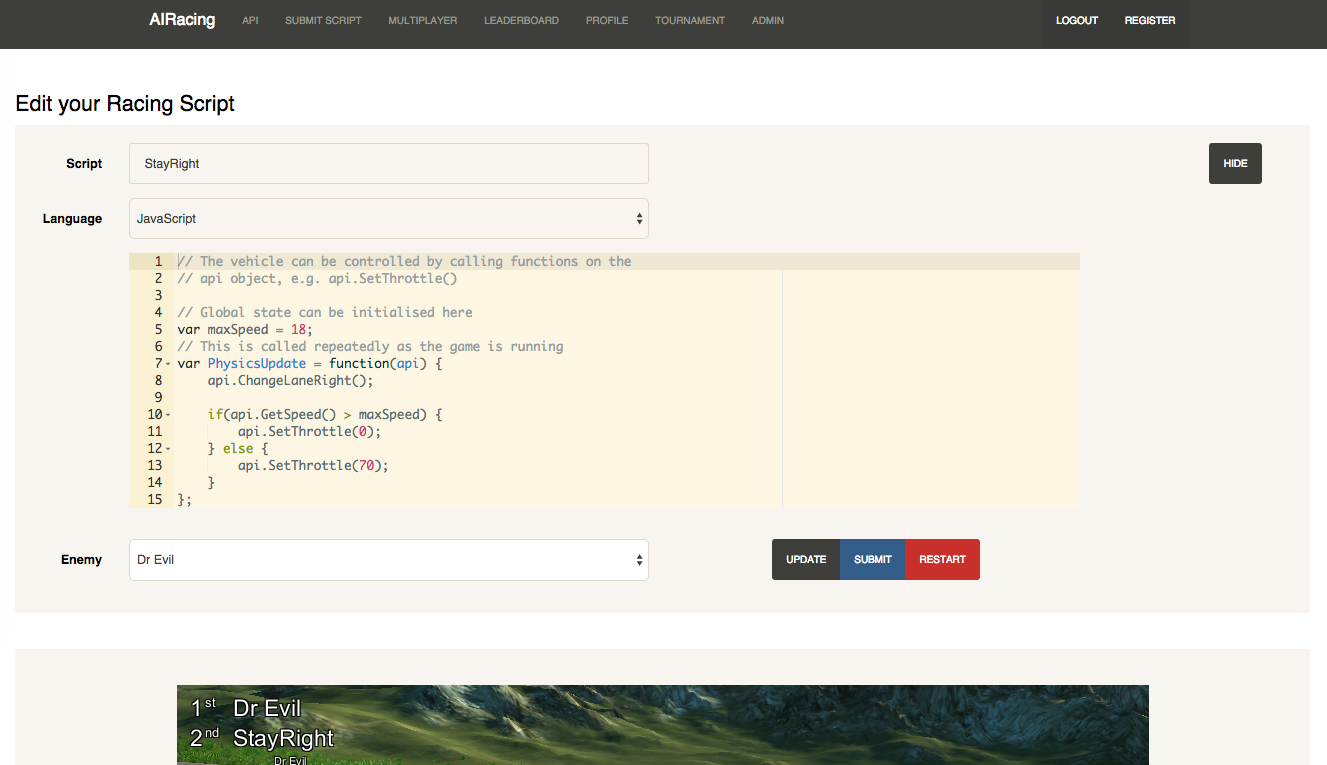
\includegraphics[width=0.49\textwidth]{editscreen.png}
	\hfill    
	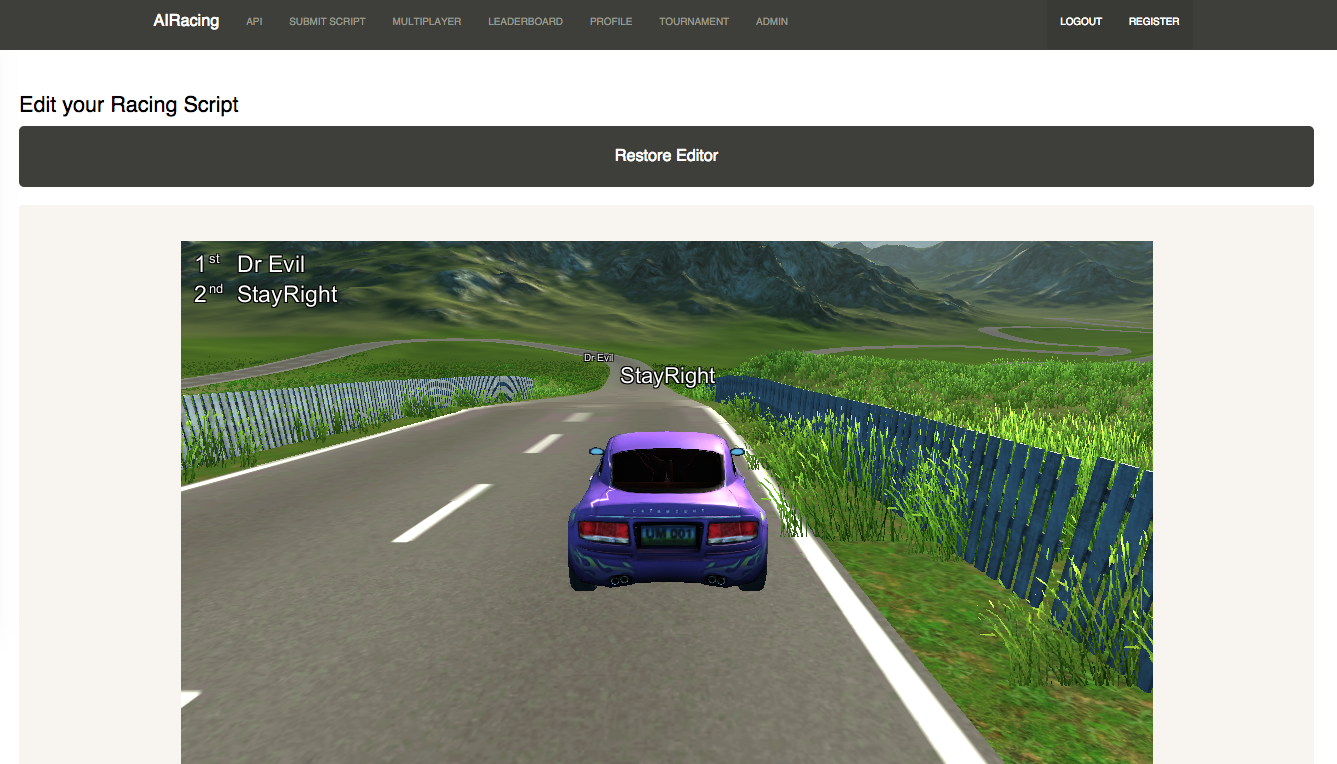
\includegraphics[width=0.49\textwidth]{editscreenhide.png}
}
\caption{Edit Screen - users can edit their scripts and test any changes made.}
\end{figure}

There are a few key differences between the script submission and editing screen, beyond the rather obvious Unity Web Player :

\begin{enumerate}
\item Hide button - Now that the user can also view their script racing alongside the Ace editor, we provided a hide button which allows the user to collapse the editing pane, displaying the race without forcing the user to scroll down the page. We decided not to display the race alongside the editor on the screen, as this either requires an unrealistically wide screen resolution, or would reduce the size of the editor and Unity web player drastically. We tested the edit screen using tabs, with the editing pane on one and the race on the other, however we experienced issues resizing the  Unity Web Player and running it in the background.
\item Restore button - After the editing pane has been collapsed, a large restore button is presented where the pane previously was. This is large to ensure that a new user does not accidentally hide the edit screen, struggle to restore it, and consequently leave the page without submitting changes. We could have used a more subtle restore button, and a  pop-up to notify the user of how to find it, but we did not want to obscure the Unity Web Player.
\item Update/Submit/Reset buttons - These new buttons are clustered together in the bottom right of the editing pane, below the Ace editor, to ensure they are visible when the computer being used has a small monitor resolution or if the web-browser has a high zoom level. Although clustering these buttons risks users accidentally submitting changes, we ensured the buttons had contrasting colours to avoid confusion.
	\begin{enumerate}
	\item Submit button - As the user is logged in, submitting changes updates the user's script and returns them to their profile. They are greeted by a pop-up that notifies them that their changes had been made successfully.
	\item Update button - Pressing the update button re-interprets the script, whether changes have been made or not. This allows the user to observe changes on demand, without restarting the race. 
	\item Reset button - Pressing the reset button restarts the race, re-interpreting the script and changing the opponent to the one selected in the ``Enemy" drop-down menu.
	\end{enumerate}
\end{enumerate}

\subsection{Admin Features}

We restricted a few features from the average user, which are only accessible by a registered admin, i.e. G-Research employee. These features were the tournament mode and admin panel, as shown below.

\begin{figure}[H]
\centering
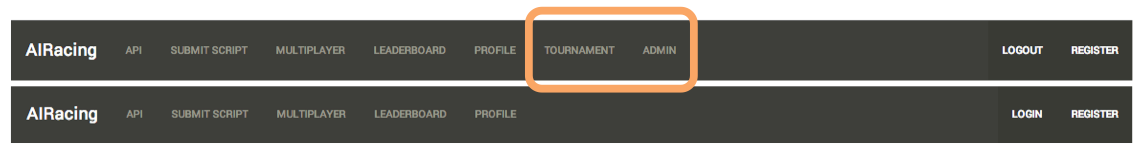
\includegraphics[width=\textwidth]{admintoolbar.png}
\caption{Admins will see additional features on their navigation bar after logging in.}
\end{figure}

These REST end points {\tt/tournament} and {\tt/admin} aren't secured from other users or anonymous users, however we do not expect users to access these features. This is mostly because users will be supervised by G-Research recruiters, but also because users will simply not know the names of these routes, and could only access them by trial and error.

The tournament button on the navigation bar will display a tournament, with races being run automatically with the leaderboard changes being displayed after each race. The admin button displays the personal details of registered users and the names of a user's scripts (shown below) - this feature was requested by our client. 
\begin{figure}[H]
\centering
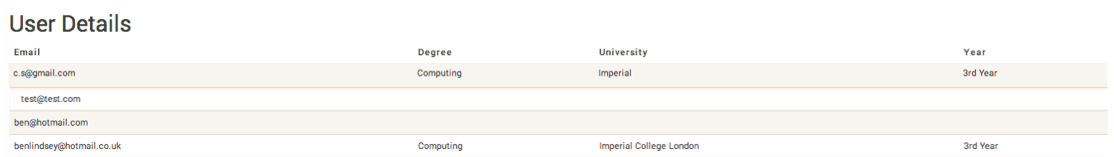
\includegraphics[width=\textwidth]{adminpanel.png}
\caption{Admins can view the details of registered users.}
\end{figure}

\section{Script Execution and Sandboxing TODO {\color{green} BEN}}
How did we convert javascript to unity script?
How do we allow global state?
Challenges to overcome: no objects. Direct control over unity objects, e.g. car teleportation. Allowing other languages.
Risks: Dr Evil!!
